\documentclass[12pt,fleqn]{article}\usepackage{../../common}
\begin{document}
Materyel Mekaniği - 6

Burulma (Torsion)

Ekşenel ve eksene dik yüklemelerden biraz daha çetrefil analiz gerektiren bir
yük uygulama şekli, bir çubuğun büküldüğü zaman ortaya çıkan burulma durumudur.
Burulma bir öğe momentlerle, ya da torklarla dönüşsel olarak yüklendiği zaman
ortaya çıkar. 

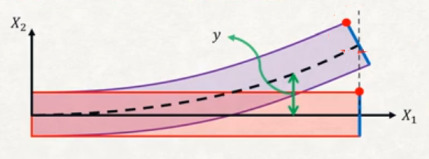
\includegraphics[width=10em]{phy_020_strs_06_01.jpg}

Mesela üstteki ilk resimde bir vidanın döndürülmesi görülüyor, bu durumda bir el
bir $T$ torku uygular. Bir arabanın tekerlek aksi, saftı ya da gemilerin
pervanesine (propeller) dönüş ileten aks aynı davranışı sergiler.  Üstte üçüncü
resimde görülen tork ilk nokta için $T_1 = P_1 d_1$ ile, ikincisi $T_2 = P_2
d_2$ ile hesaplanabilir.

Kaynaklar

[1] Bayramlı, {\em Hesapsal Bilim, Sonlu Öğeler Metotu (Finite Elements Method -FEM-), Sürekli (Continuous) Yaklaşım}

[2] Gere, {\em Mechanics of Materials}

\end{document}
